\chapter{Eksperimental Opsætning}
Denne sektion har til formål at beskrive opgavens eksperimentale opsætning og dertil hvilke billeder der er anvendt og hvordan metoderne er afprøvet.
\section{Anvendte Billeder}
De udvalgte billedsæt, som opgavens resultater bygger på, er taget fra overflyvningen af en mark. Sættene består af: 10 billeder som er taget længst væk fra jorden, 4 billeder taget næst-længst fra jorden og 4 billeder taget tættest fra jorden. I alle sættene er der traktorspor eller nedlagt korn.

\begin{figure}[H]
    \centering
    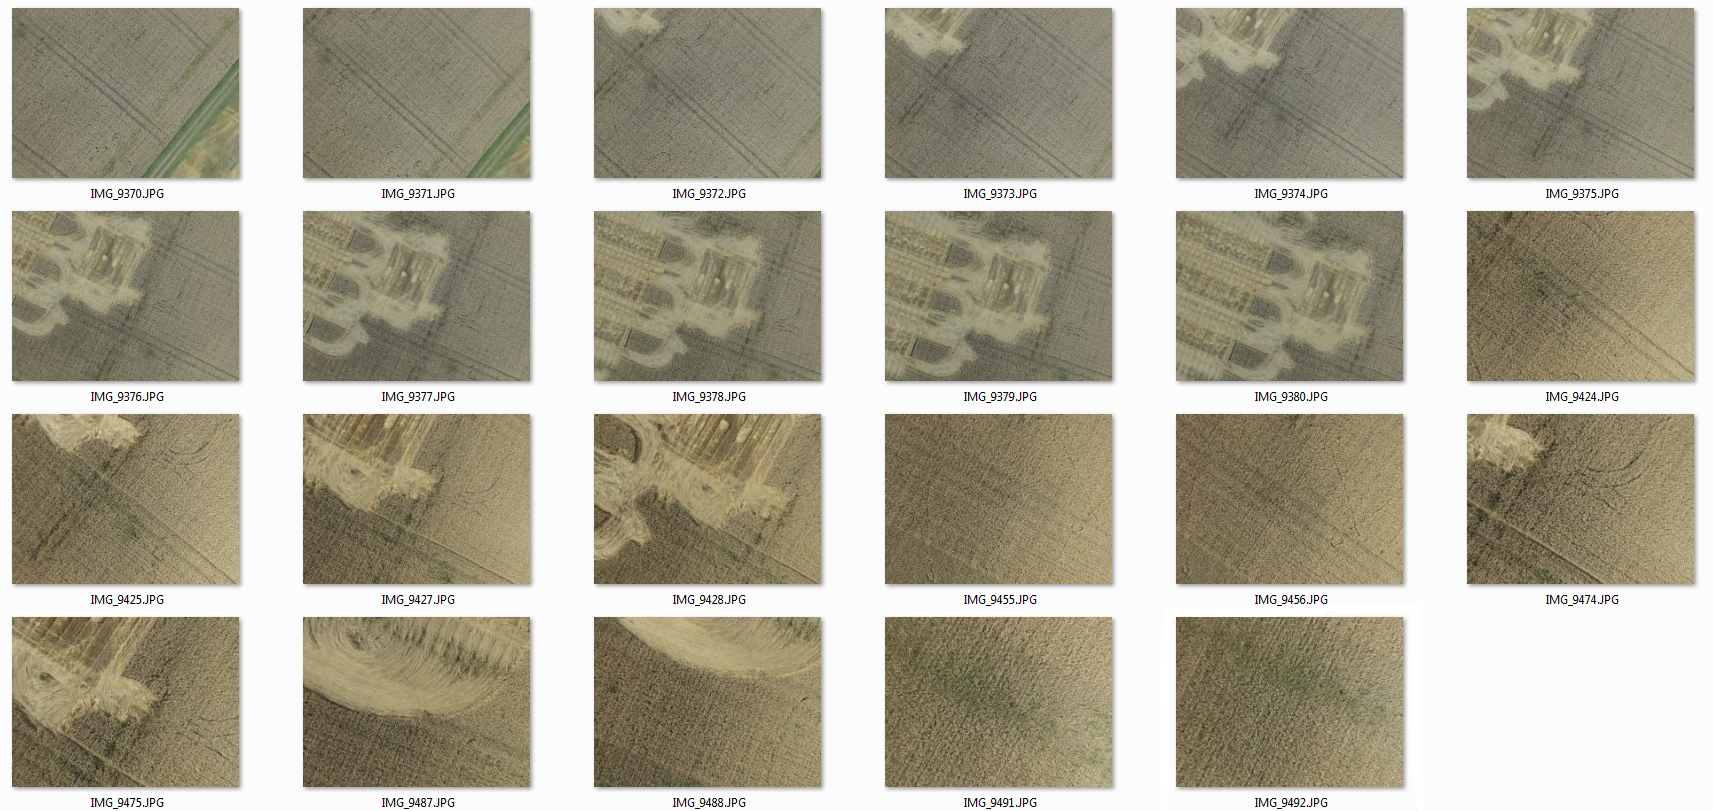
\includegraphics[width=1\textwidth]{fig/43a.png}
    \vspace{-0.5em}   
    \begin{center}
    \caption{\textcolor{gray}{\footnotesize \textit{Udvalgt billedesæt}}}
    \label{fig:lindblob}
     \end{center}
  \end{figure}
       \vspace{-2.7em}
\noindent
\section{Metode Opsætning}
Følgende er kombinationer af beskrevne metoder afprøvet på ovenstående billedsæt:
\begin{center}
    \begin{tabular}{ | l | l |}
    \hline
    Detektor & Deskriptor \\ \hline
    $DoG$ & SIFT \\ \hline       
    Harris & SIFT \\ \hline    
    Moravec & SIFT \\ \hline    
    $DoH$ & SURF\\ \hline    
    \end{tabular}
\end{center}
Da der er blevet implementeret 4 detektorer og 2 deskriptorer, er der $4\times 2=8$ mulige metoder at afprøve. Det er her begrænset til de fire ovenstående, for ikke at få drukne afsnittet i tabeller. SIFT er blevet valgt som deskriptor for metoderne, da vores undersøgelser har vist, at den giver flest matches og højest repeatability measure på de forskellige metoder, sammenlignet med SURF. 
\\
\\


<FEJLKILDER>
<test kombination af billederne> \\
<hvad er testet, rotation, struktur, skala>